\documentclass{article}
\usepackage{graphicx}
\usepackage{xcolor}
\usepackage{amsmath}
\usepackage{geometry}
\usepackage{hyperref}
\usepackage[nottoc,numbib]{tocbibind}
\usepackage[titletoc,toc,page]{appendix}
\addtocontents{toc}{\protect\thispagestyle{empty}}

\geometry{a4paper, margin=1in}

\begin{document}

% Center everything on the page
\begin{titlepage}
\begin{center}

    % Logo and title
    
\includegraphics[width=0.1\textwidth]{./resources/logo.png} \\
    \vspace{0.5cm}
    {\Huge \textbf{TikTok-Brain}} \\[0.5cm]
    {\LARGE \textit{Lo-fi Prototyping and Usability Testing}} \\[2cm]

    % Value Proposition
    \textbf{\textcolor{green}{\Large Value Proposition}} \\[0.3cm]
    \textit{\large Teamwork makes the green work.} \\[1cm]

    % Mission Statement
    \textbf{\textcolor{green}{\Large Mission Statement}} \\[0.3cm]
    \parbox{0.8\textwidth}{
        \centering
        \large
        TikTok-Brain is both a community and competition platform that empowers individuals to take sustainable actions.
    } \\[1cm]

    % Problem / Solution Overview
    \textbf{\textcolor{green}{\Large Problem / Solution Overview}} \\[0.3cm]
    \parbox{0.8\textwidth}{
        \centering
        \large
        While many people recognize the importance of sustainability, they often feel unmotivated to act sustainably when it is inconvenient to do so. TikTok-Brain taps into people’s competitiveness and desire to excel among peers to encourage sustainable living.
    } \\[1.5cm]

    % Our Team
    \textbf{\Large Our Team} \\[0.5cm]

    % Team Photos and Names
    \begin{tabular}{ccc}
        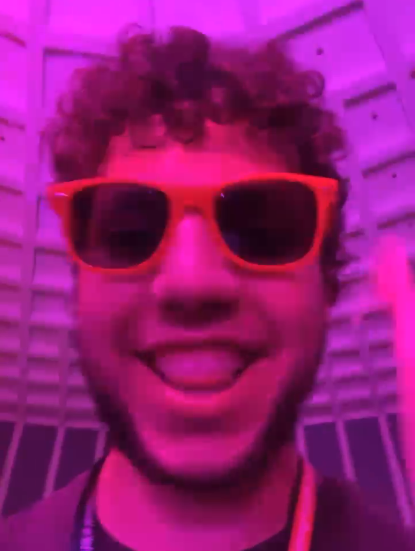
\includegraphics[width=0.2\textwidth]{./resources/ole.png} &
        
\includegraphics[width=0.2\textwidth]{./resources/markus.png} &
        
\includegraphics[width=0.2\textwidth]{./resources/diba.png} \\[0.3cm]
        Ole Einar Grundmann & Markus Siegert & Diba Zokai \\
    \end{tabular}
\end{center}
\end{titlepage}

\newpage
\tableofcontents
\newpage

\section{Introduction}
Provide an introduction to the project, discussing the background, motivation, and objectives of your work. Describe the problem in more detail and explain why sustainability is crucial.

\section{Methodology}
This section explains the methodology used in your project. Break it down into subsections for clarity.

\subsection{Research and Planning}
Discuss your research, planning process, and the steps taken to prepare for prototyping and usability testing.

\subsection{Prototyping}
Explain the process of creating the low-fidelity prototype. Include diagrams or wireframes if available:
\begin{figure}[h!]
    \centering
    \includegraphics[width=0.8\textwidth]{prototype.png} % Replace with path to prototype image
    \caption{Lo-fi Prototype of TikTok-Brain Platform}
    \label{fig:prototype}
\end{figure}

\subsection{Usability Testing}
Describe the usability testing process, including how you gathered participants, conducted tests, and collected feedback.

\section{Results}
Present the results of your project in this section. You might want to use tables, charts, and figures to show the data clearly.

\begin{table}[h!]
    \centering
    \begin{tabular}{|c|c|c|}
        \hline
        Metric & Prototype & Feedback Score \\
        \hline
        Usability & 4.5 & Positive \\
        Sustainability Awareness & 4.2 & Neutral \\
        Engagement & 4.8 & Very Positive \\
        \hline
    \end{tabular}
    \caption{Usability Testing Results}
    \label{tab:results}
\end{table}

\section{Discussion}
Analyze the results here, discussing what the results imply about the effectiveness of your platform. Discuss any limitations or challenges encountered.

\section{Conclusion}
Summarize the key findings and discuss the impact of your work. Outline potential future work or improvements for the platform.

\newpage
\bibliographystyle{ieeetr}
\bibliography{Bibliography}
\newpage

\renewcommand{\thesection}{\Alph{section}}

\appendix

\section{AI Appendix}
asdf

\end{document}
